\documentclass{article}

\usepackage[utf8]{inputenc}
\usepackage[T1]{fontenc}
\usepackage[spanish]{babel}

\usepackage{caratula}
\usepackage{caption}
\usepackage{hyperref}
\usepackage{graphicx}
\usepackage{amsmath}
\usepackage{amsfonts}
\usepackage{minted}
\usepackage{tikz}
\usepackage[most]{tcolorbox}
\usepackage{multicol}
\usepackage[a4paper, total={7.25in, 10in}]{geometry}

% anexo-codigo: se añaden todos los .cpps al PDF
% anexo-links: se añade un link a cada problema
\def\versionanexo{anexo-codigo}

\hypersetup{
    colorlinks=true,
    linkcolor=blue,
    filecolor=blue,      
    urlcolor=blue,
    pdftitle={Treaps},
    pdfpagemode=FullScreen,
    }

\captionsetup[figure]{hypcap=false}

\setlength{\parindent}{0pt}
\setlength{\parskip}{4pt}
\setcounter{tocdepth}{2}

\usetikzlibrary{shapes.multipart}
\usetikzlibrary {arrows.meta}

\newtcolorbox{Pbox}{
enhanced,
colback=white,
}

\newcommand\problema[1]{\begin{Pbox}#1\end{Pbox}}
\newcommand\member[1]{\!\!\rightarrow\!\! \text{#1}}

\titulo{Treaps}
\subtitulo{Aumentando Árboles de Búsqueda Binaria para Competencias}
\materia{Programación Competitiva II}
\submateria{Lucas Hernán Tarche}
\integrante{}{}{}

\begin{document}

\maketitle
\tableofcontents
\newpage

\begin{multicols*}{2}

\section{Introducción}

En la literatura, muchos problemas pueden ser resueltos adaptando un árbol de búsqueda binaria balanceado, como es el caso de un Árbol AVL o Árbol Red-Black.
Sin embargo, la implementación de ambas estructuras es larga y con varios casos, lo que no es óptimo para competencias.
En su lugar, presentamos el Treap o Árbol de Búsqueda Binaria Aleatorio, cuya implementación es simple y concisa,
y mantiene el tiempo esperado con una muy alta probabilidad.

Vamos a usar esta estructura para resolver varios problemas de competencia,
así como mostrar técnicas y trucos para aumentar árboles binarios,
incluyendo "Treap Implícito" para manipulado de secuencias, y cómo añadirle persistencia a la estructura.

\section{Preliminares}

\subsection{Árboles de Búsqueda Binaria (ABBs)}

Un árbol de búsqueda binaria o ABB es una estructura que permite guardar los elementos
de un conjunto finito totalmente ordenado \(X\), es decir,
que todo par de elementos \(x, y \in X\), es \textit{comparable}, es decir, exactamente uno de los siguientes es verdadero: 

\[ x < y \qquad x = y \qquad  x > y \]

En cada nodo $x$ del árbol se guarda un valor del conjunto, y posee además dos hijos (potencialmente nulos),
llamados izquierdo y derecho, con la propiedad que el hijo izquierdo es un ABB del conjunto
$X_< = \{ y \in X : y < x \}$; y el hijo derecho es un ABB del conjunto $X_> = \{y \in X : y > x\}$.
Notar que no pueden haber dos nodos con el mismo valor, por cómo se definen estos conjuntos.

En nuestro caso, $X$ va a ser un subconjunto de \( \mathbb{Z} \), el conjunto de números enteros.
Podemos pensar que cada nodo del ABB representa un intervalo,
de manera que cada nivel del árbol (los nodos a una cierta profundidad) es una partición de \(\mathbb{Z}\) menos los elementos que hay en niveles superiores.

\begin{center}
\begin{tikzpicture}[
sibling distance=1.25in,
every node/.style={draw}
]
\node {\(7: (-\infty, \infty)\)}
    child { node {\(3: (-\infty, 7)\)} }
    child { node {\(11: (7, \infty)\)} 
        child { node {\(8: (7, 11)\)}
            child [missing]
            child { node {\(9: (8, 11)\)}}
        }
        child { node {\(13: (13, \infty)\)}}
    };
\end{tikzpicture}
\captionof{figure}{Particionar niveles en intervalos}
\end{center}

\vbox{
El árbol soporta tres operaciones sobre el conjunto:

\begin{enumerate}
    \item Buscar(\(x\)), que dice si \(x\) pertenece o no al conjunto
    \item Insertar(\(x\)), que inserta \(x\) en el conjunto
    \item Borrar(\(x\)), que elimina \(x\) del conjunto
\end{enumerate}
}

Estas tres operaciones cuestan $\mathcal{O}(h)$,
donde $h$ es la máxima profundidad de un nodo (también llamada la altura del árbol).
Como cada nivel $k$ tiene a lo sumo $2^k$ nodos, $h \geq \lceil \lg |X| \rceil$.
En el peor de los casos, puede ocurrir que $h = n$.

Por esta razón, existen los Árboles de Búsqueda Binaria Auto-Balanceables,
que garantizan que \(h = \mathcal{O}(\lg n)\), como el caso de árboles AVL o Red-Black.
En el caso del Treap, se realiza esta misma cota con muy alta probabilidad.

\subsection{Heaps}

Un \textit{Heap} (binario), también conocido como "Montículo", es otra clase de árbol binario,
que guarda un valor en cada nodo, y mantiene la propiedad que todo nodo tiene
el valor máximo en su subárbol.

\begin{center}
\begin{tikzpicture}[
every node/.style={circle,draw}
]
\node {\(19\)}
    child {node {\(17\)}
        child {node {\(2\)}}
        child {node {\(7\)}}
    }
    child {node {\(3\)}};
\end{tikzpicture}
\captionof{figure}{Ejemplo de un Heap}
\end{center}

Se pueden insertar y eliminar nodos en $\mathcal{O}(\lg n)$, y acceder al máximo elemento en tiempo constante.
Sin embargo, en nuestro caso, no nos va a interesar usarlo como estructura de datos,
sino que vamos a usar la forma del árbol determinada por los valores.

\section{Treap}

Un \textit{Treap}, también conocido como Árbol de Búsqueda Binaria Aleatoreizado, es un ABB, en el que guardamos en cada nodo \(x\) una clave \(x_v\), y
un valor auxiliar llamado la \textit{prioridad} del nodo, \(x_p\). 
Estas prioridades cumplen la misma propiedad que los valores de un Heap, es decir, que la prioridad máxima de un subárbol
se encuentra en la raíz de dicho subárbol.

Si al momento de insertar un nuevo nodo, le asignamos una prioridad aleatoria,
la altura esperada del árbol resulta ser logarítmica. En particular, para toda constante \(c \in \mathbb{R}_{>0}\), la probabilidad que la altura sea mayor a \(2c \ln n\) está acotada por:

\[
\mathbb{P}[h \geq 2c \ln n] < n(n/e)^{-c \ln(c/e)}
\]

Por ejemplo, si \(n = 200000\), la probabilidad que la altura sea mayor a \(4 \ln n\) es menor que \(0.006\).

Además, si \(x\) es un nodo cualquiera, su profundidad esperada es \(\mathbb{E}[x] < 1 + 2 \ln n\). 
Por lo tanto, casi seguramente el Treap va a funcionar casi igual de rápido que otros árboles, que tienen garantías sobre la complejidad, y esto se confirma en la práctica.

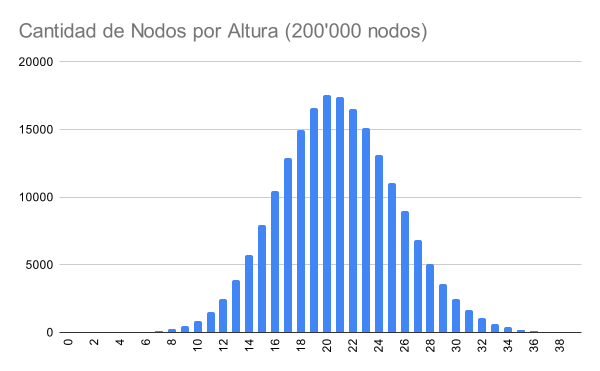
\includegraphics[width=0.8\linewidth]{Diagramas/distribucion_nodos.png}

Hay dos formas equivalentes de implementar el Treap, por eso vamos a optar por la más simple, que deriva todas las operaciones de implementar Split / Merge.

\subsection{Split}
Split(\(T, k\)) toma un Treap \(T\) y una clave \(k\), y retorna dos Treaps, \(T_\leq\) y \(T_>\), tales que:

\begin{itemize}
\item \(T_\leq \cup T_> = T\)
\item \(\forall x \in T_\leq, x_v \leq k\)
\item \(\forall x \in T_>, x_v > k\)
\end{itemize}

Es decir, particiona el Treap en dos con respecto a \(k\).
Este método va a funcionar en \(\mathcal{O}(\lg n)\) \footnote{Dado que el Treap se construye de manera aleatoria, vamos a hablar de complejidad \textit{esperada}.}, y consiste en recorrer el árbol, comparando el nodo actual con \(k\).

Si el valor en la raíz es menor o igual que \(k\), entonces la raíz y todo su subárbol izquierdo tienen que estar en \(T_\leq\), entonces partimos el subárbol derecho con respecto a \(k\), y juntamos ambas partes.
Sino, es análogo, porque la raíz y todo su subárbol derecho deben estar en \(T_>\), entonces sólo falta partir el subárbol izquierdo.

\vbox{
\begin{minted}{c++}
pair<Treap, Treap> split(Treap root, int k) {
  if (root == nullptr) return {nullptr, nullptr};
  
  if (root->key <= k) {
    auto [left, right] = split(root->right, k);
    root->right = left;
    return {root, right};
  } else {
    auto [left, right] = split(root->left, k);
    root->left = right;
    return {left, root};
  }
}
\end{minted}
}

\subsection{Merge}

De manera análoga a Split(), Merge(\(T_L, T_R\)) toma dos Treaps, el izquierdo con todos los elementos menores al derecho, y retorna un Treap con los nodos de ambos.

Tenemos que asegurar que esta operación mantenga cierto que las prioridades tienen forma de Heap.
Para esto, colocamos de raíz a la raíz del Treap con mayor prioridad.
En el caso que sea el izquierdo, hay que juntar el hijo derecho con el Treap derecho, para mantener 
el orden relativo de los nodos, para poder buscarlos a futuro.
El caso del hijo derecho es análogo, poniendo al árbol derecho de raíz, y llamando Merge() entre el árbol izquierdo, y el subárbol izquierdo del derecho.

\vbox{
\begin{minted}{c++}
Treap merge(Treap left, Treap right) {
  if (left == nullptr) return right;
  if (right == nullptr) return left;

  if (left->priority > right->priority) {
    left->right = merge(left->right, right);
    return left;
  } else {
    right->left = merge(left, right->left;
    return right;
  }
}
\end{minted}
}

Cabe destacar que, tanto Split como Merge invalidan los Treaps anteriores. 
Sin embargo, mediante \hyperref[sec:persistencia]{persistencia}, es posible mantener válidos los Treaps de input, al costo de tener que crear \(\mathcal{O}(\lg n)\) nodos adicionales.

\subsection{Insertar y Borrar}

Para insertar un nodo con valor \(x\) en el árbol, vamos a llamar a Split() dos veces,
para obtener los árboles \(T_<\), \(T_=\) y \(T_>\) (potencialmente vacíos), 
con los nodos menores, iguales o mayores que \(x\), respectivamente.

Si \(T_=\) tiene un nodo, este tiene valor igual a \(x\), y no hay que insertar nada, entonces simplemente juntamos \(T_<\) con \(T_>\).
Sino, reemplazamos \(T_=\) por un nodo nuevo con valor \(x\) (un nodo solo es a su vez un árbol),
y juntamos \(T_<\) con \(T_=\), y el resultado con \(T_>\).

Similarmente, si queremos eliminar un nodo con valor \(x\), llamamos a Split() de la misma forma,
y juntamos \(T_<\) con \(T_>\). 
Dependiendo de si el lenguaje de implementación posee un \textit{Garbage Collector} o no, puede hacer falta eliminar manualmente el nodo en \(T_=\).

\subsection[Construcción en O(n)]{Construcción en \(\mathcal{O}(n)\)}

Claramente, se puede construir un Treap en \(\mathcal{O}(n \lg n)\), 
simplemente llamando a Insert() \(n\) veces.
Sin embargo, si ya tenemos ordenados los valores iniciales a insertar, es posible reducirlo a tiempo lineal.

Primero creamos un Árbol de Búsqueda Binaria balanceado, partiendo la lista de elementos a la mitad, y llamando recursivamente. Esto es \(\mathcal{O}(n)\), ya que hacemos una cantidad constante de operaciones por nodo.

Como puede ocurrir que las propiedades no cumplan la propiedad de Heap, ahora tenemos una segunda etapa, en la que hacemos Heapify() sobre las prioridades, lo que cuesta \(\mathcal{O}(n)\), 
por ejemplo usando el algoritmo \textit{BuildHeap} de Floyd.

Nota: Incluso si los elementos no están ordenados, suele ser más rápido ordenarlos y crearlo de esta manera, porque tiene menor constante, y la altura inicial del árbol es exactamente \(\lceil \lg n \rceil\).


\section{Aumentando Árboles Binarios}

Hasta ahora, el único uso que le podemos dar al Treap es como Conjunto / Diccionario. 
Esto no es útil para competencias, porque existen en las bibliotecas estándar implementaciones de estos tipos de datos. 
Por ejemplo, en C++ se puede usar \texttt{std::set} o \texttt{std::map}, respectivamente.

La idea va a ser \textit{aumentar} el árbol, almacenando información adicional en los nodos, para poder hacer operaciones más interesantes. 

\subsection[Árbol de Estadísticos de Orden (Order Statistics Tree)]{Árbol de Estadísticos de Orden \newline (Order Statistics Tree)}
\label{sec:order-statistics-tree}

Un Árbol de Estadísticos de Orden es un ABB, que además soporta las siguientes operaciones:

\begin{enumerate}
    \item Select(\(k\)), que retorna el \(k\)-ésimo elemento más chico.
    \item Rank(\(x\)), que devuelve la cantidad de elementos menores o iguales a \(x\).
\end{enumerate}

A la respuesta de Select(\(k\)) también se la llama \(k\)-ésimo estadístico de orden. Además, si \(x\) está en el conjunto, Rank(\(x\)) nos dice que número de estadístico de orden es \(x\).

Ambas operaciones van a funcionar en \(\mathcal{O}(\lg n)\), pero vamos a tener que guardar un parámetro adicional: el \textit{tamaño} de un subárbol.

Para cada nodo \(x\), definimos su tamaño como:
\[
|x| = |x_L| + |x_R| + 1
\]
donde \(x_L\) y \(x_R\) son sus hijos izquierdo y derecho.
Además, si un nodo \(x\) es nulo, decimos que su tamaño es cero.

Este valor adicional se puede mantener calculándolo al momento de creación, y actualizando un nodo cada vez que cambia alguno de sus hijos.
Para esto, podemos cambiarlo en Split() y Merge() cuando estamos por devolver el nuevo árbol.

\begin{center}
\begin{tikzpicture}[
level 1/.style={sibling distance=2in},
level 2/.style={sibling distance=1in},
level 3/.style={sibling distance=0.5in},
every node/.style={
    circle split,
    draw
}
]

\node { 26 \nodepart{lower} 7 }
    child {
        node { 17 \nodepart{lower} 4 }
        child { node { 4 \nodepart{lower} 1 } }
        child {
            node { 21 \nodepart{lower} 2 }
            child { node { 19 \nodepart{lower} 1} }
            child [missing]
        }
    }
    child {
        node { 41 \nodepart{lower} 2 }
        child { node { 30 \nodepart{lower} 1 } }
        child [missing]
    }
;
\end{tikzpicture}
\captionof{figure}{Clave y tamaño en un Order Statistics Tree}
\end{center}

\subsubsection{Select()}

Vamos a recorrer el árbol desde la raíz, comparando los tamaños con el \(k\) buscado.
Si el hijo izquierdo tiene exactamente \(k - 1\) nodos, entonces la respuesta es la raíz. Si tiene más de \(k - 1\), está en el hijo izquierdo, así que llamamos recursivamente. Finalmente, si tiene menos de \(k - 1\) nodos, la respuesta debe estar en el subárbol derecho, y llamamos a Select(\(k - |x_L| - 1\)) sobre el subárbol derecho.

\vbox{
\begin{minted}{c++}
int select(Treap root, int k) {
  if (size(root->left) == k - 1) return root->value;
  if (size(root->left) > k - 1) {
    return select(root->left, k);
  } else {
    k -= size(root->left) + 1;
    return select(root->right, k);
  }
}
\end{minted}
}

\subsubsection{Rank()}

Para implementar Rank(), partimos el Treap con respecto a \(x\), usando Split(). La respuesta es el tamaño de \(T_\leq\), lo único es que hay que recordar llamar a Merge() antes de retornar.

\subsection{SPOJ - Ghost Town}

\problema{
\textbf{Ghost Town:}

Queremos un multiconjunto que soporte:

\begin{enumerate}
\item Count(\(x\)): retorna cantidad de valores \(\leq x\)
\item Select(\(k\)): retorna el \(k\)-ésimo valor más chico
\item Insert(\(x\) + Count(\(x\)))
\end{enumerate}

En todos los casos, los elementos se cuentan con repeticiones.
Por ejemplo, Select(\(\{1, 1, 2\}, 2\)) = 1.

\url{https://www.spoj.com/problems/COUNT1IT/}
}

Notar que, si en lugar de un multiconjunto pidiera un conjunto, sería simplemente implementar un Order Statistics Tree.
Aunque es tentador que nuestra implementación permita nodos con valores repetidos, esto nos da de peor caso \(h = \mathcal{O}(n)\), insertando siempre el mismo elemento\footnote{Esto es similar a ciertas implementaciones de Quicksort, que resultan \(\mathcal{O}(n^2)\) si todos los elementos son iguales.}.

En su lugar vamos a guardar en cada nodo la cantidad de veces que aparece su valor en el multiconjunto, y lo notamos \(x_f\). Es suficiente cambiar nuestra definición de tamaño a

\[|x| = |x_L| + |x_R| + |x_f|\]

así como modificar ligeramente la implementación de Select(), y sumarle uno a \(x_f\) al insertar un valor repetido.

\subsection{SPOJ - Ada and Harvest}

\problema{
\textbf{Ada and Harvest:}

Tenemos una lista \(a_1, \dots, a_n\) de números, y queremos responder \(q\) consultas del tipo ``contar cuántos números en \(a_1, ..., a_{k - 1}\) iguales a \(x\), y luego reemplazar \(a_k\) por \(x\)''.

\url{https://www.spoj.com/problems/ADACROP/}
}

Vamos a tratar de adaptar el problema para poder usar un Order Statistics Tree.
Notar que dos números distintos en la lista ``no interactúan'' entre sí, porque al momento de responder para \(x\), 
sólo nos interesan las posiciones con valor igual a \(x\).

\begin{center}
\begin{tikzpicture}[scale=0.7]
\draw (0,0) grid (10,1);

\node at (0.5,0.5) {$2$};
\node at (1.5,0.5) {$3$};
\node at (2.5,0.5) {$5$};
\node at (3.5,0.5) {$3$};
\node at (4.5,0.5) {$9$};
\node at (5.5,0.5) {$3$};
\node at (6.5,0.5) {$5$};
\node at (7.5,0.5) {$2$};
\node at (8.5,0.5) {$9$};
\node at (9.5,0.5) {$9$};

\footnotesize
\node at (0.5,1.4) {$1$};
\node at (1.5,1.4) {$2$};
\node at (2.5,1.4) {$3$};
\node at (3.5,1.4) {$4$};
\node at (4.5,1.4) {$5$};
\node at (5.5,1.4) {$6$};
\node at (6.5,1.4) {$7$};
\node at (7.5,1.4) {$8$};
\node at (8.5,1.4) {$9$};
\node at (9.5,1.4) {$10$};

\normalsize
\draw (1,-1) grid (3, -2);
\node at (1.5, -1.5) {$1$};
\node at (2.5, -1.5) {$8$};

\footnotesize
\node at (0.5, -1.5) {$2$:};

\normalsize
\draw (6,-1) grid (9, -2);
\node at (6.5, -1.5) {$2$};
\node at (7.5, -1.5) {$4$};
\node at (8.5, -1.5) {$6$};

\footnotesize
\node at (5.5, -1.5) {$3$:};

\normalsize
\draw (1,-3) grid (3, -4);
\node at (1.5, -3.5) {$3$};
\node at (2.5, -3.5) {$7$};

\footnotesize
\node at (0.5, -3.5) {$5$:};

\normalsize
\draw (6,-3) grid (9, -4);
\node at (6.5, -3.5) {$5$};
\node at (7.5, -3.5) {$9$};
\node at (8.5, -3.5) {$10$};

\footnotesize
\node at (5.5, -3.5) {$9$:};

\end{tikzpicture}
\captionof{figure}{Descomposición en índices del ejemplo}
\end{center}

Por esta razón, vamos a armar un árbol por cada valor, y guardamos los índices 
en los que aparece este valor en la lista actual. 
Aunque esto parezca costoso, vamos a ver a lo sumo \(n + q\) valores distintos, y podemos guardar los árboles en un diccionario.

Ahora, responder una consulta es buscar el árbol apropiado y llamar a Rank(\(k\)), y después sacar \(k\) del árbol viejo, y añadirlo al nuevo. Por lo tanto, la complejidad es \(\mathcal{O}((n + q) \lg (n + q))\).

\section{Range Queries}

Muchos problemas de estructuras de datos consisten en calcular una función acumulada sobre un rango de un arreglo, como la suma de elementos en el intervalo \([l, r]\).
Es decir, si nuestro arreglo es \(a_1, \dots, a_n\), queremos calcular 

\[
f(l, r) = a_l + a_{l + 1} + \dots + a_r = \sum_{i = l}^r{a_i}
\]

En general, esto vale para cualquier \textbf{monoide}.
Decimos que una operación binaria \(\oplus\) sobre un conjunto \(A\) es un monoide si es:

\begin{itemize}
\item Cerrada: si \(a, b \in A\), \(a \oplus b \in A\)
\item Asociativa: \((a \oplus b) \oplus c = a \oplus (b \oplus c)\) para todos \(a, b, c \in A\)
\item Elemento neutro: existe un (único) elemento \(e \in X\) tal que \(e \oplus a = a \oplus e = a\) para todo \(a \in A\)
\end{itemize}

Hay varios ejemplos comunes de monoides, incluyendo la suma, el producto, máximo y mínimo, entre otros. 
De hecho, ambas definiciones para el tamaño de un nodo eran monoides.

De manera similar al tamaño, definimos para cada nodo \(x\) la función acumulada en su subárbol como

\[
f(x) = f(x_L) \oplus x_a \oplus f(x_R)
\]

donde \(f\) de un nodo nulo es la identidad del monoide \(\oplus\), y \(x_a \in A\) es algún valor asociado a \(x\).
En el caso del tamaño, \(x_a\) era la frecuencia del valor.

Para usar un Treap para resolver esta clase de problemas, insertamos las claves \(1, \dotsm, n\), cada una con su valor original. 
De esta forma, computar \(f(l, r)\) se reduce a dos llamados de Split(), para obtener los elementos con clave en \([l, r]\), y la respuesta es la función acumulada de la raíz:

\vbox{
\begin{minted}{c++}
int query(Treap &root, int l, int r) {
    Treap left, middle, right;
    tie(left, right) = split(root, r);
    tie(left, middle) = split(left, l - 1);
    
    int ans = f(middle);
    root = merge(merge(left, middle), right);
    return ans;
}
\end{minted}
}

\subsection{CSES - Dynamic Range Sum Queries}
\label{sec:dynamic-range-sum-queries}
\problema{
\textbf{Dynamic Range Sum Queries:}

Tenemos una lista con números \(a_1, \dots, a_n\), y queremos responder \(q\) consultas del tipo: 
\begin{enumerate}
    \item Cambiar \(a_k\) por \(x\)
    \item Computar la suma en \([l, r]\)
\end{enumerate}

\url{https://cses.fi/problemset/task/1648}
}

Como la suma es un monoide (cuya identidad es cero), ya sabemos computar sumas en rango de manera eficiente.
Para cambiar el valor en una posición, particionamos el árbol en tres con respecto a \(k\), actualizamos el valor, y juntamos todo de nuevo.

\vbox{
\begin{minted}{c++}
void update(Treap &root, int k, int x) {
    Treap left, middle, right;
    tie(left, right) = split(root, k);
    tie(left, middle) = split(left, k - 1);

    middle->value = x;
    root = merge(merge(left, middle), right);
}
\end{minted}
}

Tanto Update() como Query() funcionan en \(\mathcal{O}(\lg n)\), entonces la complejidad de la solución es \(\mathcal{O}(n + q \lg n)\). 

\subsection{CSES - Range Updates and Sums}

\problema{
\textbf{Range Updates and Sums:} 

Tenemos una lista de números \(a_1, \dots, a_n\), y queremos responder \(q\) consultas del tipo:
\begin{enumerate}
\item Sumarle \(x\) a cada elemento en \([l, r]\)
\item Reemplazar por \(x\) cada elemento en \([l, r]\)
\item Computar la suma en \([l, r]\)
\end{enumerate}

\url{https://cses.fi/problemset/task/1735/}
}

Notar que, si directamente aplicáramos las operaciones de tipos 1. y 2. apenas llegan,
la cantidad de posiciones a cambiar es \(\mathcal{O}(n \cdot q)\), que son demasiadas operaciones para las cotas del problema.
En su lugar, vamos a marcar que tenemos que actualizar un subárbol, e ir propagando las actualizaciones cuando visitamos un nodo (un truco conocido como \textit{Lazy Propagation}).

Para poder hacer Lazy Propagation, necesitamos:
\begin{itemize}
    \item Una forma de computar la función acumulada de un nodo, incluso si tiene actualizaciones pendientes
    \item Una forma de componer actualizaciones
    \item Una forma de aplicar las actualizaciones pendientes a un nodo, y propagarlas a sus hijos
\end{itemize}

En cada nodo, vamos a guardar tres valores adicionales, que representan las actualizaciones que tiene pendientes:
un entero diciendo cuánto hay que añadirle al subárbol (\texttt{lazyAdd}), un entero diciendo cuánto hay que asignarle a cada nodo del subárbol (\texttt{lazySet}), y un booleano que dice si hay que hacer una asignación o no. 
Este último parámetro es necesario, ya que no existe una ``identidad'' para asignar valores.

Para computar la función acumulada de un nodo, tenemos dos casos, dependiendo de si hay o no una actualización de reemplazo pendiente.

Si tenemos que realizar una asignación:
\[
f(x) = |x| \cdot (x \member{lazyAdd} + x \member{lazySet})
\]

Caso contrario, es igual a:
\[
f(x) = f(x_L) + f(x_R) + x_a + |x| \cdot x \member{lazyAdd}
\]

Para componer con una actualización de suma, le sumamos la cantidad a \texttt{lazyAdd}.
Por otro lado, si queremos componer con un reemplazo, tenemos que reemplazar \texttt{lazyAdd} por cero, y asignarle a \texttt{lazySet} el nuevo valor.

Finalmente, para propagar actualizaciones, el valor del nodo es \(x \member{lazySet} + x \member{lazyAdd} \) si hay que asignar, y \(x_a + x \member{lazyAdd}\) si no.

De manera similar al problema anterior, para hacer una actualización hay que buscar el rango afectado con Split(), y componer con la nueva actualización. 
Solo es necesario propagar las actualizaciones necesarias cuando visitamos un nodo en Split() o Merge():

\begin{minted}{c++}
pair<Treap, Treap> split(Treap root, tint k) {
  if (root == nullptr) return {nullptr, nullptr};

  propagate(root);
  if (root->key <= k) // ...
}

Treap merge(Treap left, Treap right) {
  if (left == nullptr) return right;
  if (right == nullptr) return left;

  propagate(left), propagate(right);
  if (left->priority > right->priority) // ...
}
\end{minted}

Como sólo hacemos una cantidad constante de operaciones adicionales en Split() y Merge(), la complejidad de este problema también es \(\mathcal{O}(n + q \lg n)\).


\section{Treap Implícito}

Vamos a ver un truco particularmente útil para manipular secuencias y cadenas,
conocido como ``Treap Implícito'' o ``Treap con Claves Implícitas''. 
A diferencia de los problemas que vimos hasta ahora, los tres problemas a continuación no
pueden resolverse usando alguna variante de Segment Tree.

Un patrón clásico en problemas es añadir consultas de cortar/pegar y/o invertir rangos,
para evitar usar un Segment Tree, como es el caso de \nameref{sec:reversals-and-sums}.
En su lugar, debe aumentarse un ABB autobalanceado, siendo Treap y Splay Tree
los dos más populares para competencias.

\subsection{CSES - Cut and Paste}

\problema{
\textbf{Cut and Paste:} 

Tenemos una cadena \(S = s_1 \dots s_n\), y vamos a cortar una subcadena \(s_l \dots s_r\) y pegarla al final \(q\) veces.

Imprimir la cadena después de todas las operaciones.

\url{https://cses.fi/problemset/task/2072}
}

Notar que, luego de una operación, pasamos de la cadena \(S = s_1 \dots s_n\) a la cadena \(S' = s_1 \dots s_{l - 1} s_{r + 1} \dots s_n s_l \dots s_r\).
Es decir, partimos \(S\) en tres porciones, y las pegamos en una nueva cadena. 
Uno querría insertar los pares índice, carácter en un Treap, de manera similar que para sumas, 
y usar Split() y Merge() para cortar y pegar, respectivamente.

Lamentablemente, esto no funciona, porque luego de una operación, el árbol podría dejar de tener la propiedad de búsqueda binaria, así como que las claves ya no representen los índices:

\begin{center}
\begin{tikzpicture}[
sibling distance=0.5in,
every node/.style={
    circle split,
    draw
}
]

\node { R \nodepart{lower} 2 }
    child { node { T \nodepart{lower} 1 } }
    child {
        node { A \nodepart{lower} 4 }
        child { node { E \nodepart{lower} 3 } }
        child { node { P \nodepart{lower} 5 } }
    }
;
\end{tikzpicture}
\begin{tikzpicture}[
sibling distance=0.5in,
every node/.style={
    circle split,
    draw
}
]

\node { R \nodepart{lower} 2 }
    child { node { T \nodepart{lower} 1 } }
    child {
        node { E \nodepart{lower} 3 }
        child { node { P \nodepart{lower} 5 } }
        child { node { A \nodepart{lower} 4 } }
    }
;
\end{tikzpicture}
\captionof{figure}{Intentando hacer ``TREAP'' \(\to\) ``TRPEA''}
\end{center}

Queremos alguna forma de actualizar todos los índices cuando cortamos el árbol,
pero sin tener que recorrer los nodos uno por uno.
Para evitar esto, la idea va a ser no guardarnos las claves en el árbol,
sino deducirlas en el momento con la estructura del árbol.

Definimos la \textit{clave implícita} de un nodo como su posición en el inorder de recorrer el árbol desde la raíz.
Aunque no estén almacenados explícitamente en cada nodo, los podemos obtener a medida que vamos recorriendo 
el árbol para hacer Split(). 
Hay que modificar ligeramente Split() para que funcione con claves implícitas:

\vbox{
\begin{minted}{c++}
pair<Treap, Treap> split(Treap root, int k) {
 if (root == nullptr) return {nullptr, nullptr};
  
 int key = size(root->left) + 1;
 Treap left, right;
 if (key <= k) {
  tie(left, right) = split(root->right, k - key);
  root->right = left;
  evaluate(root);
  return {root, right};
 } else {
  tie(left, right) = split(root->left, k);
  root->left = right;
  evaluate(root);
  return {left, root};
 }
}
\end{minted}
}

Como los nodos no tienen claves, no hay que mantener su orden, entonces podemos pegar árboles que, conceptualmente, no están en órden. 
Esta propiedad hace que la implementación sea lo que habíamos pensado originalmente:

\vbox{
\begin{minted}{c++}
void update(Treap &root, int l, int r){
  Treap left, middle, right;
  tie(left, right) = split(root, r);
  tie(left, middle) = split(left, l - 1);
  root = merge(merge(left, right), middle);
}
\end{minted}
}

Finalmente, imprimir el resultado es concatenar los caracteres de los nodos en recorrido inorder, y la complejidad total es \(\mathcal{O}(n + q \lg n)\).

\subsection{CSES - Substring Reversals}
\problema{
\textbf{Substring Reversals:} 

Tenemos una cadena \(S = s_1 \dots s_n\), y vamos a dar vuelta subcadenas \(s_l \dots s_r\) un total de \(q\) veces.

Imprimir la cadena después de todas las operaciones.

\url{https://cses.fi/problemset/task/2073}
}

Vamos a armar un Treap Implícito con los caracteres, de la misma forma que en el problema anterior. 
Notar que, si no fuera implícito, podría romperse el orden de las claves luego de una actualización.

Recordemos que, para invertir un árbol binario, intercambiamos los hijos izquierdo y derecho de la raíz, y procedemos recursivamente.
Además, invertir dos veces un árbol nos devuelve el árbol original.
Esto nos da la idea de usar Lazy Propagation para procesar rápido las actualizaciones, sin tener que recorrer todos los nodos afectados.

Sólo hace falta guardarse un booleano adicional por nodo,
que nos indica si hay una actualización pendiente o no.
El resultado es sorprendente porque, si omitimos imprimir la respuesta, podemos dar vuelta una subcadena en \(\mathcal{O}(\lg n)\).
Obtener la cadena final es cuestión de recorrer el árbol en recorrido inorder, propagando actualizaciones a medida que visitamos los nodos.

\begin{center}
\begin{tikzpicture}[
sibling distance=0.5in,
every node/.style={
    circle,
    draw
}
]
\node[fill=lightgray] { R \nodepart{lower} 2 }
    child { node { T } }
    child {
        node { A }
        child { node { E } }
        child { node { P  } }
    }
;
\end{tikzpicture}
\begin{tikzpicture}[
sibling distance=0.5in,
every node/.style={
    circle,
    draw
}
]
\node { R \nodepart{lower} 2 }
    child {
        node[fill=lightgray] { A }
        child { node { E } }
        child { node { P  } }
    }
    child { node[fill=lightgray] { T } }
;
\end{tikzpicture}
\begin{tikzpicture}[
sibling distance=0.5in,
every node/.style={
    circle,
    draw
}
]
\node { R \nodepart{lower} 2 }
    child {
        node { A }
        child { node[fill=lightgray] { P  } }
        child { node[fill=lightgray] { E } }
    }
    child { node { T } }
;
\end{tikzpicture}
\captionof{figure}{Dar vuelta ``TREAP'' \(\to\) ``PAERT''}
\end{center}

\subsection{CSES - Reversals and Sums}
\label{sec:reversals-and-sums}

\problema{
\textbf{Reversals and Sums:} 

Tenemos una lista de números \(a_1 \dots a_n\), y queremos responder \(q\) consultas del tipo:

\begin{enumerate}
\item Dar vuelta el rango \([l, r]\)
\item Computar la suma en el rango \([l, r]\)
\end{enumerate}

\url{https://cses.fi/problemset/task/2074}
}

La solución a este problema es casi inmediata, sólo tenemos que combinar la respuesta al problema anterior con la solución a \nameref{sec:dynamic-range-sum-queries}.
Esto es fácil de hacer, ya que no cambia la suma de un subárbol al invertirlo.

De este problema, podemos notar lo siguiente:
\begin{itemize}
\item Podríamos haber usado claves implícitas para resolver los problemas de Range Queries.
\item Es fácil añadirle consultas de cortar/pegar o invertir rangos a un problema de Range Queries, si tenemos una solución con Treap.
\end{itemize}

De hecho, podríamos haber resuelto el problema ``Range Updates, Sums and Reversals'' de la misma forma.

\section{Persistencia}
\label{sec:persistencia}

Una estructura de datos se dice \textit{persistente} si preserva sus estados anteriores, incluso después de realizarle actualizaciones.
En lugar de modificar los valores almacenados en cada nodo, lo que vamos a hacer es crear ``clones'' de los nodos a cambiar, con las modificaciones necesarias ya aplicadas.
De esta forma, como no se modificó ningún valor, no se invalida una representación vieja al hacer actualizaciones.

En el caso del Treap, sólo vamos a crear \(\mathcal{O}(\lg n)\) nodos adicionales por llamado a Split() / Merge(), y es cuestión de reemplazar asignaciones por crear nodos nuevos.

Detalle de implementación: como puede ser difícil llevar cuenta de qué punteros tenemos que borrar en cada momento,
es conveniente usar punteros inteligentes (\texttt{std::shared\_ptr}), para que la memoria se libere cuando no es usada.

\begin{minted}{c++}
pair<Treap, Treap> split(Treap root, int k) {
 if (root == nullptr) return {nullptr, nullptr};

 Treap left, right;
 if (root->key <= k) {
  left = make_shared<Node>(*root);
  tie(left->right, right) = split(root->right, k);
  evaluate(left);
 } else {
  right = make_shared<Node>(*root);
  tie(left, right->left) = split(root->left, k);
  evaluate(right);
 }
 return {left, right};
}

Treap merge(Treap left, Treap right) {
 if (left == nullptr) return right;
 if (right == nullptr) return left;

 Treap root;
 if (left->priority > right->priority) {
  root = make_shared<Node>(*left);
  root->right = merge(left->right, right);
 } else {
  root = make_shared<Node>(*right);
  root->left = merge(left, right->left);
 }
 evaluate(root);
 return root;
}
\end{minted}

Persistencia todavía no es un tema común en competencias, y menos todavía Treaps Persistentes.
Sin embargo, nos permite hacer en \(\mathcal{O}(\lg n)\) operaciones que la intuición dice no deberían ser posibles, como llamar a Merge() de parte de un árbol con sí mismo,
usando otro truco conocido como ``Treap con Prioridades Implícitas''.

\subsection{SWERC 2020 - H. Figurines}
\problema{
\textbf{H. Figurines:} (resumido)

Tenemos un conjunto, inicialmente vacío, y los números \(1, \dots n\).
A lo largo de \(n\) días, vamos a insertar y eliminar estos números, cada uno exáctamente una vez.

Responder \(q\) consultas, del tipo ``¿Cuántos elementos mayores o iguales que \(x\) había en el conjunto, al finalizar el día \(d\)?''.

\url{https://codeforces.com/gym/103081/problem/H}
}

La solución al problema es usar un \hyperref[sec:order-statistics-tree]{Order Statistics Tree} Persistente para resolver el problema.
Primero, queremos generar los \(n\) árboles, insertando y removiendo del árbol apropiado.
Luego, es cuestión de procesar las consultas en orden, llamando a Rank() en el Treap con índice \(d\).

Nota: esta versión resumida del problema puede resolverse sin usar persistencia, pues podemos ordenar las consultas por día, de manera que sólo hay un árbol activo a la vez.
En el problema original esto no es posible, porque el valor \(x\) de cada consulta depende de la respuesta a la consulta anterior.

\subsection{CodeChef - GENETICS}
\problema{
\textbf{GENETICS:}

Tenemos \(n\) cadenas de ADN \(D_1, \dots D_n\) (palabras con letras A, C, G, T),
y podemos realizar tres tipos de operaciones sobre las mismas:

\begin{enumerate}
\item Combinar(\(i_1, i_2, k_1, k_2\)): 

Añade las cadenas \(D_{i_1}[1 .. k_1] + D_{i_2}[k_2+1 ..]\) y \(D_{i_2}[1 .. k_2] + D_{i_1}[k_1+1..]\) al final de la lista

\item Mutar(\(i, k, c\)): Cambia el carácter en la posición \(k\) de \(D_i\) por \(c\)
\item Contar(\(i, l, r\)): Devuelve la frecuencia de cada carácter en \(D_i[l..r]\)
\end{enumerate}

Se garantiza que no se van a producir cadenas de longitud mayor a \(2 \cdot 10^9\).

\url{https://www.codechef.com/problems/GENETICS}
}

Notar que la cota sobre la longitud máxima es importante, porque podemos duplicar el tamaño de la cadena más larga en un paso con un llamado a Combinar().

\begin{center}
\begin{tikzpicture}[xscale=0.65, yscale=-0.65]

\normalsize
\fill[red!20](0,0) rectangle (6, 1);
\fill[blue!20](6,0) rectangle (10, 1);
\draw (0,0) grid (10,1);
\node at (0.5,0.5) {A};
\node at (1.5,0.5) {T};
\node at (2.5,0.5) {G};
\node at (3.5,0.5) {G};
\node at (4.5,0.5) {C};
\node at (5.5,0.5) {G};
\node at (6.5,0.5) {A};
\node at (7.5,0.5) {A};
\node at (8.5,0.5) {A};
\node at (9.5,0.5) {G};

\footnotesize
\node at (-0.5,0.5) {$D_1$:};

\normalsize
\fill[blue!20](0,2) rectangle (4, 3);
\fill[red!20](4,2) rectangle (10, 3);
\draw (0,2) grid (10,3);
\node at (0.5,2.5) {A};
\node at (1.5,2.5) {G};
\node at (2.5,2.5) {A};
\node at (3.5,2.5) {C};
\node at (4.5,2.5) {A};
\node at (5.5,2.5) {T};
\node at (6.5,2.5) {G};
\node at (7.5,2.5) {C};
\node at (8.5,2.5) {A};
\node at (9.5,2.5) {A};

\footnotesize
\node at (-0.5,2.5) {$D_2$:};

\normalsize
\fill[red!20](-1,4) rectangle (11, 5);
\draw (-1, 4) grid (11, 5);
\node at (-0.5,4.5) {A};
\node at (0.5,4.5) {T};
\node at (1.5,4.5) {G};
\node at (2.5,4.5) {G};
\node at (3.5,4.5) {C};
\node at (4.5,4.5) {G};
\node at (5.5,4.5) {A};
\node at (6.5,4.5) {T};
\node at (7.5,4.5) {G};
\node at (8.5,4.5) {C};
\node at (9.5,4.5) {A};
\node at (10.5,4.5) {A};

\footnotesize
\node at (-1.5, 4.5) {$D_3$:};

\normalsize
\fill[blue!20](1,6) rectangle (9, 7);
\draw (1, 6) grid (9, 7);
\node at (1.5,6.5) {A};
\node at (2.5,6.5) {G};
\node at (3.5,6.5) {A};
\node at (4.5,6.5) {C};
\node at (5.5,6.5) {A};
\node at (6.5,6.5) {A};
\node at (7.5,6.5) {A};
\node at (8.5,6.5) {G};

\footnotesize
\node at (0.5, 6.5) {$D_4$:};
\end{tikzpicture}
\captionof{figure}{Ejemplo de Combinar()}
\end{center}

Del diagrama podemos ver que Combinar() es cortar en dos las cadenas originales, y pegarlas para obtener una cadena nueva.
Por esta razón, vamos a representar cada cadena con un Treap Persistente con claves implícitas, y procedemos de la forma que muestra el diagrama.

Para hacer los llamados a Mutar(), vamos a sobrescribir la posición en la lista de cadenas
con el resultado de sacar el nodo viejo en la posición \(k\), e insertar el nuevo.
No podemos modificar directamente el nodo, porque podrían verse afectadas otras cadenas que apunten a ese nodo o algún antecesor.

Para los llamados a Contar(), mantenemos en cada nodo como función acumulada una tupla, que representa la frecuencia de cada carácter, 
y obtener la respuesta es igual que otros problemas de Range Queries.

Por lo tanto, la complejidad temporal es \(\mathcal{O}(n |s| + q \lg L)\), donde \(|s|\) es la longitud máxima de una cadena del input (en este caso, 30000), 
y \(L\) es la longitud máxima que puede tener una cadena.

\subsection{Petrozavodsk Summer Training Camp 2017 - C. Sequence}

\problema{
\textbf{C. Sequence:}

Tenemos un array \(A = a_1 \dots a_n\), y tres tipos de operaciones:
\begin{enumerate}
\item Computar la suma en el rango \([l, r]\)
\item Correr el siguiente pseudocódigo:

\texttt{for (l <= i <= r) a[i] = a[i - k];}
\item Asignar \(a_i = a'_i\) para todo \(i \in [l, r]\)
\end{enumerate}

Donde \(A' = a'_1 \dots a'_n\) son los valores originales de \(A\).

\url{https://www.acmicpc.net/problem/19068}
}

Vamos a usar un Treap con claves implícitas para mantener las sumas de rangos, queremos ver cómo soportar las otras dos operaciones.
Además, necesitamos un cierto nivel de persistencia, pero en un momento dado sólo nos interesan dos árboles: el original, y el actual.

Las operaciones de tipo 3. son relativamente simples, tenemos que usar Split() para conseguir el rango [l, r] del árbol original, y reemplazarlo en el Treap actual:

\begin{minted}{c++}
Treap toCopy 
  = split(split(orig, r).first, l - 1).second;
auto [left, right] = split(root, r);
left = split(left, l - 1).first;
root = merge(merge(left, toCopy), right);
\end{minted}

El verdadero problema son las operaciones de tipo 2., que no es inmediato ver como evitar correr el pseudocódigo. 
Esto se debe a que, como los rangos de inicio y llegada pueden intersecarse, no es necesariamente reemplazar el rango \([l - k, r - k]\) en la posición \([l, r]\).

\begin{center}
\begin{tikzpicture}[xscale=0.7, yscale=-0.7]

\draw (0,0) grid (10,1);
\node at (0.5,0.5) {$1$};
\node at (1.5,0.5) {$2$};
\node at (2.5,0.5) {$3$};
\node at (3.5,0.5) {$4$};
\node at (4.5,0.5) {$5$};
\node at (5.5,0.5) {$6$};
\node at (6.5,0.5) {$7$};
\node at (7.5,0.5) {$8$};
\node at (8.5,0.5) {$9$};
\node at (9.5,0.5) {$10$};

\draw[arrows={->}] (5, 1.1) -- (5, 1.9);
\node at (7.2, 1.5) {$l = 5, r = 9, k = 2$};

\draw (0,2) grid (10,3);
\node at (0.5,2.5) {$1$};
\node at (1.5,2.5) {$2$};
\node at (2.5,2.5) {$3$};
\node at (3.5,2.5) {$4$};
\node at (4.5,2.5) {$3$};
\node at (5.5,2.5) {$4$};
\node at (6.5,2.5) {$3$};
\node at (7.5,2.5) {$4$};
\node at (8.5,2.5) {$3$};
\node at (9.5,2.5) {$10$};

\end{tikzpicture}
\captionof{figure}{Ejemplo de operación tipo 2}
\end{center}

Luego de observar un par de ejemplos, podemos ver que estamos repitiendo el rango \([l - k, l - 1]\) varias veces, y colocándolo en el rango \([l, r]\).
Podemos duplicar la longitud del rango con cada llamado a Merge(), y cada llamado cuesta \(\mathcal{O}(\lg n)\), entonces podemos responder estas consultas en \(\mathcal{O}(\lg^2 n)\).

Hay un pequeño detalle: las prioridades que se obtienen al juntar un árbol con sí mismo ya no son aleatorias.
Esto se vuelve evidente cuando \(k = 1\), porque tenemos un único nodo, entonces la estructura del árbol es una lista enlazada, que tiene altura \(n\).

La solución a este problema es un truco conocido como ``prioridades implícitas''.
En lugar de guardar un valor aleatorio en cada nodo expresando su prioridad,
al momento de juntar dos nodos en Merge(), vamos a elegir \(L\) con probabilidad \(\frac{|L|}{|L| + |R|}\), y \(R\) el resto de los casos.

Puede demostrarse que estos dos métodos (prioridades explícitas e implícitas) generan los mismos árboles con la misma probabilidad, 
entonces la complejidad esperada sigue siendo \(\mathcal{O}(\lg n)\).
Podríamos haber usado prioridades implícitas para resolver todos los problemas,
pero necesitamos generar más números (pseudo-)aleatorios en total, lo que nos da una peor constante.

Por lo tanto, la complejidad esperada del problema es \(\mathcal{O}(n + q \lg^2 n))\).

\section{Conclusión}

Logramos resolver una gran variedad de problemas con Treap, y es una estructura que puede ser útil tener en el \textit{notebook} del equipo para la ICPC.
Sorprendentemente, todas las técnicas vistas pueden ser aplicadas a cualquier árbol balanceado que tenga implementado los métodos Split() y Merge().
Dado que el Treap es no determinista, hay equipos y participantes que utilizan en su lugar estructuras amortizadas, siendo las más populares Splay Tree y 2-3 Trees,
que también son más simples de implementar que una estructura determinista.

Hay otras técnicas de Segment Trees, como ``Segment Tree Beats'' para sumas y cambiar a máximo en rango, que también aplican al Treap, como en el siguiente problema: \url{https://codeforces.com/gym/102787/problem/D}, 
o mantener el hash polinómico / \textit{rolling hash} de una cadena, como en \url{https://codeforces.com/gym/102787/problem/B}.

Aunque pareciera que todo problema de Segment Tree pueda resolverse con Treap,
la constante del Treap (o cualquier otro árbol binario balanceado) puede ser muy grande,
y que el código sea más largo puede llevar a bugs en competencias.

\end{multicols*}

\newpage
\appendix

\section{Anexo}

\input{Secciones/\versionanexo}

\section{Bibliografía}

\begin{itemize}
\item Randomized Search Trees - Raimund Seidel y Cecilia R. Aragon: \url{https://faculty.washington.edu/aragon/pubs/rst96.pdf}
\item Randomized Binary Search Trees - Conrado Martínez y Salvador Roura: \url{https://dl.acm.org/doi/10.1145/274787.274812}
\item Fast Set Operations Using Treaps - Guy E. Blelloch y Margaret Reid-Miller: \url{https://www.cs.cmu.edu/~scandal/papers/treaps-spaa98.pdf}
\item Introduction to Algorithms - Cormen, Leiserson, Rivest y Stein
\item Persistent / Immutable Treaps - Blog de Ankit Sultana: \url{https://ankitsultana.com/2021/03/29/persistent-treaps.html}
\item Página sobre Treaps de CP-Algorithms: \url{https://cp-algorithms.com/data_structures/treap.html}
\item AlgorithmsThread 9: Treaps! - Video de SecondThread: 
\url{https://www.youtube.com/watch?v=6x0UlIBLRsc}
\item Training Camp Argentina 2022 - Charla de Marcos Kolodny: \url{https://www.youtube.com/watch?v=LAVptsKXbjI}
\end{itemize}

\end{document}
